\documentclass[reqno,12pt]{amsart}
\usepackage{amsmath}
\usepackage{amssymb}
\usepackage{tikz}
\usetikzlibrary{shapes.geometric}

\begin{document}

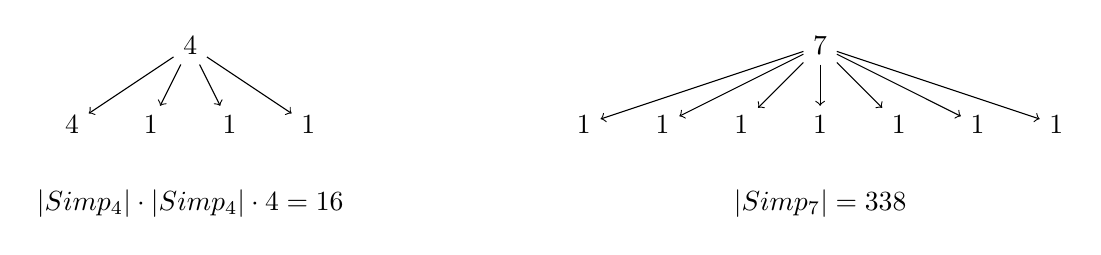
\begin{tikzpicture}
       \tikzstyle{every node} = [rectangle]
      
         \node (4) at (-4,1) {$4$};
            \node (41) at (-5.5,0) {$4$};
            \node (42) at (-4.5,0) {$1$};
            \node (43) at (-3.5,0) {$1$};
            \node (44) at (-2.5,0) {$1$};
           
          \node (exp4) at (-4,-1) {$|Simp_4| \cdot |Simp_4| \cdot 4 = 16$};
          
       
        \node (7) at (4,1) {$7$};
            \node (71) at (1,0) {$1$};
            \node (72) at (2,0) {$1$};
            \node (73) at (3,0) {$1$};
            \node (74) at (4,0) {$1$};
            \node (75) at (5,0) {$1$};
            \node (76) at (6,0) {$1$};
            \node (77) at (7,0) {$1$};
            
          \node (exp7) at (4,-1) {$|Simp_7|=338$};  
            
        \foreach \from/\to in {4/41,4/42,4/43,4/44,7/71,7/72,7/73,7/74,7/75,7/76,7/77}
            \draw[->] (\from) -- (\to);
    \end{tikzpicture}

\end{document}